\documentclass{article}
\usepackage[utf8]{inputenc}
\usepackage{longtable}
\usepackage[a4paper, margin=1in]{geometry}
\usepackage{amsmath}
\usepackage{amssymb}
\usepackage{pifont}
\usepackage{pdflscape}
\usepackage{graphicx}
\usepackage{xcolor}
\usepackage{adjustbox}
\usepackage{hyperref}

\input{filters}
\input{units}

\title{SOAP -- Spherical Overdensity and Aperture Processor}
\author{Rob McGibbon, Bert Vandenbroucke, John Helly, \\Joop Schaye, Matthieu Schaller}
\date{}

\begin{document}

\maketitle

\input{timestamp}

\section{Introduction}

SOAP computes properties for different types of halos, which differ in how they decide
on which particles to included (by radius, in projection...). SOAP does not identify
halos itself, instead it uses the halo centre and the boundedness of particles as determined
by an input subhalo catalogue (such as HBT-HERONS, SubFind, etc...).
The purpose of this file is to document the catalogues output by SOAP. For information about running
the code you should refer to the README at \href{https://github.com/SWIFTSIM/SOAP}{https://github.com/SWIFTSIM/SOAP}.
This documentation is generated using the SOAP parameter file, and so the halo types and properties 
listed reflect those present in the current run of SOAP, rather than all possible properties.
If you have any questions regarding the halo types or properties mentioned in the document then
please send an email to \href{mailto:mcgibbon@strw.leidenuniv.nl}{mcgibbon@strw.leidenuniv.nl}.
It would be useful for us to know which parts of the document need clarifying.

SOAP catalogues are output as HDF5 files, with the properties being grouped by halo type.
For loading the catalogues we recommend using the swiftsimio package. A simple example is:
\begin{verbatim}
import swiftsimio as sw
base_dir = '/cosma8/data/dp004/flamingo/Runs'
run = 'L1000N1800/HYDRO_FIDUCIAL'
data = sw.load(f'{base_dir}/{run}/SOAP-HBT/halo_properties_0077.hdf5')
# Load a dataset
m200 = data.spherical_overdensity_200_crit.total_mass
# Specify units
m200.convert_to_units('Msun')
# Specify physical/comoving
m200.convert_to_physical()
# Get metadata from file
z = data.metadata.redshift
\end{verbatim}

\section{Particle selection for different halo types}

SOAP computes properties for many different definitions of halo types. The halo type defines how to select the
particles to use when computing the properties. There are two decisions to be made - firstly whether
to include particles which are unbound. Secondly whether to exclude particles which are outside of a certain
aperture.

\paragraph{Subhalo quantities (SH)} are computed for each subhalo identified by the halo finder, irrespective of whether 
it is a central or a satellite (or even satellite of satellite and so on). They include all particles
that they halo finder has determined are bound to the subhalo. Subhalo properties are contained within the group 
\verb+BoundSubhalo+ in the output file.

\paragraph{Exclusive sphere quantities (ES)} are similar to subhalo quantities as they include only the 
particles that are bound to the subhalo, but they apply an additional radial cut (aperture). Exclusive sphere 
properties are contained within a group \verb+ExclusiveSphere/XXXkpc+, where 
\verb+XXX+ is the corresponding \textbf{physical} aperture radius.

\paragraph{Inclusive sphere quantities (IS)} use a physical aperture radii cut the same as the exclusive sphere 
quantities. However for the inclusive sphere we include all particles within the radius, regardless of their 
membership status. If the aperture radius of an inclusive sphere variation is greater than the EncloseRadius
(the maximum distance between a bound particle and the halo centre) of a subhalo, then for that subhalo no
properties are computed for the variation.
The quantities are stored within the group \verb+InclusiveSphere/XXXkpc+. 

\paragraph{Exclusive projected quantities (EP)} are similar to exclusive sphere quantities, except that their 
aperture cut is applied in projection. For each radii there are three  independent projections: along the 
x-, y- and z-axis. Along the projection axis, we do not apply any radial cut, meaning the depth corresponds to all particles 
bound to the subhalo. Projected aperture quantities are stored in a group named 
\verb+ProjectedAperture/XXXkpc/projP+, where \verb+XXX+ is the corresponding aperture radius, and \verb+P+ 
corresponds to a particular projection direction (\verb+x+, \verb+y+ or \verb+z+).

\paragraph{Spherical overdensity properties (SO)} are fundamentally different from the three other types in 
that their aperture radius is determined from the density profile and is different for different halos. They 
always include all particles within a sphere around the halo centre, regardless of halo membership. 
The radius is either the radius at which the density reaches a certain target value (e.g.  200 
crit, 100 crit, 200 mean, BN98) or a multiple of such a radius (5xR 500 crit). Details 
of the spherical overdensity calculation are given in section \ref{sec:so_calculation}. Spherical overdensities are 
only computed for central subhalos, i.e. field halos. The quantities are stored in a group 
\verb+SO/XXX+, where \verb+XXX+ can be either \verb+XXX_mean+ for density multiples of the mean density, 
\verb+XXX_crit+ for density multiples of the critical density, \verb+BN98+ for the overdensity definition of 
Bryan \& Norman (1998), or \verb+YxR_XXX_ZZZ+ for multiples of some other radius (e.g. \verb+5xR_2500_mean+). 
The latter can only be computed after the corresponding density multiple SO radius has been computed. This is 
achieved by ordering the calculations.

\paragraph{InputHalos} Some properties are directly copied from the original halo catalogue that was passed
to SOAP. These are stored in a separate group, \verb+InputHalos+.

\paragraph{SOAP} Some properties are computed by SOAP using the other halo properties present in the catalogue.
These are stored in a separate group, \verb+SOAP+. This is just done for convenience; these quantities could be computed from the SOAP output alone.

\paragraph{The table below lists} all the groups in the output file which containing datasets.
Note that there will be three groups (\verb+x+, \verb+y+ or \verb+z+) for each \verb+ProjectedAperture+ variation.
Each halo variation can have a filter applied to it. If a subhalo does not satisfy the filter then the halo variation
will be skipped for that subhalo, and all properties will have a value of zero. More information on filters can be found in the next section.

\input{variations_table}

\section{Filters}

Halo properties only make sense if the subhalo contains sufficient particles. Halo finders are often run with a 
configuration that requires at least 20 particles for a subhalo. 
However, even for those particle numbers, a lot of the properties computed by SOAP will be zero (e.g. 
the gas mass within a 10 kpc aperture), or have values that are outliers compared to the full halo population 
because of undersampling. We can save a lot of disk space by filtering these out by applying appropriate cuts. 
Filtering means setting the value of the property to zero; HDF5 file compression then very effectively 
reduces the data storage required to store these properties, while the size of the arrays that the end user 
sees remains unchanged. We also save on computing time by not computing properties that are 
filtered out.

Since different properties can have very different requirements, and so each property has a filter associated
with it. These filters are consistent across different halos types for the same property, e.g. the properties
for an inclusive sphere with a 10 kpc aperture radius will use the same filters as the quantities of the inclusive 
sphere with a 3000 kpc aperture radius, even 
though the latter by construction has many more particles.

\paragraph{Basic quantities (basic)} are never filtered out, and hence are calculated for all objects in the
input halo catalogue.

\paragraph{General quantities (general)} use a filter based on the total number of particles bound to the 
subhalo.

\paragraph{Gas quantities (gas)} use a filter based on the number of gas particles bound to the subhalo. 

\paragraph{DM quantities (dm)} use a filter based on the number of DM particles bound to the subhalo.

\paragraph{Stellar quantities (star)} use a filter based on the number of star particles bound to the 
subhalo.

\paragraph{Baryon quantities (baryon)} use a filter based on the number of gas and star particles 
bound to the subhalo.

\paragraph{}Note that there are no quantities that use a BH or neutrino particle number filter.
The different categories are summarised in the table below.

\begin{longtable}{ll}
Name & criterion \\
\hline{}basic & (all halos) \\
general & $N_{\rm{}gas}+N_{\rm{}dm}+N_{\rm{}star}+N_{\rm{}BH} \geq{} \generalfilter$ \\
gas & $N_{\rm{}gas} \geq{} \gasfilter$ \\
dm & $N_{\rm{}dm} \geq{} \dmfilter$ \\
star & $N_{\rm{}star} \geq{} \starfilter$ \\
baryon & $N_{\rm{}gas}+N_{\rm{}star} \geq{} \baryonfilter$ \\
\end{longtable}

\section{Property table}

The table below lists all the properties that are computed by SOAP when run in HYDRO mode.
For dark matter only (DMO) mode only the properties coloured violet/purple are computed.
This table is automatically generated by SOAP from the source code and parameter file, so that all
names, types, units, categories and descriptions match what is actually
used and output by SOAP.
Superscript numbers refer to more detailed explanations for some of the properties and match the numbers in
the next section. If swiftsimio has been used to load a catalogue then the fields names are in snake\_case rather
than CamelCase, e.g. \verb+CentreOfMass+ becomes \verb+centre_of_mass+. For each quantity, the table
indicates for which halo types the property is computed. If a property is being calculated 
for a certain halo type it is marked with a \ding{51}. Properties calculated
for snapshots but not snipshots are indicated with a \ding{36}.

\paragraph{}Note that quantities are output in the base units of the simulation snapshot. 
We therefore recommend that swiftsimio is used to load the catalogues as it has unit handling built in.
However, the attributes of each SOAP dataset do contain all the relevant meta-data to convert between physical
and co-moving units, i.e. information about how the
quantity depends on the scale-factor, and what the conversion factor to and from CGS units is. \textbf{All quantities
are $h$-free.} The conversion of the base units to CGS is given by:

\begin{longtable}{cl}
Unit & CGS conversion \\
\hline{}
L & \lengthbaseunit      \hspace{1mm} cm \\
M & \massbaseunit        \hspace{1mm} g \\
t & \timebaseunit        \hspace{1mm} s \\
T & \temperaturebaseunit \hspace{1mm} K \\
\end{longtable}

For example, a property whose units are listed as L/t will have units of velocity,
where $1 \, \rm{L/t} = \velbaseunit \, \rm{km/s}$.
The scale factor is explicitly included for comoving properties (e.g. the units of HaloCentre are
listed as aL).

\input{table}

\section{Non-trivial properties}

\input{footnotes}

\section{Spherical overdensity calculations}
\label{sec:so_calculation}

The radius at which the density reaches a certain threshold value is found by linear interpolation of the 
cumulative mass profile obtained after sorting the particles by radius. The approach we use is different from 
that taken by VR, where both the mass and the radius are obtained from independent interpolations on the mass 
and density profiles (the latter uses the logarithm of the density in the interpolation). The VR approach is 
inconsistent, in the sense that the condition

\begin{equation}
    \frac{4\pi{}}{3} R_{\rm{}SO}^3 \rho{}_{\rm{}target} = M_{\rm{}SO},\label{eq:MSO_condition}
\end{equation}

is not guaranteed to be true, and will be especially violated for large radial bins (the bins are generated 
from the particle radii by sorting the particles, so we have no control over their width). We instead opt to 
guarantee this condition by only finding $R_{\rm{}SO}$ or $M_{\rm{}SO}$ by interpolation and using eq. 
(\ref{eq:MSO_condition}) to derive the other quantity.

\begin{figure}
    \centering
    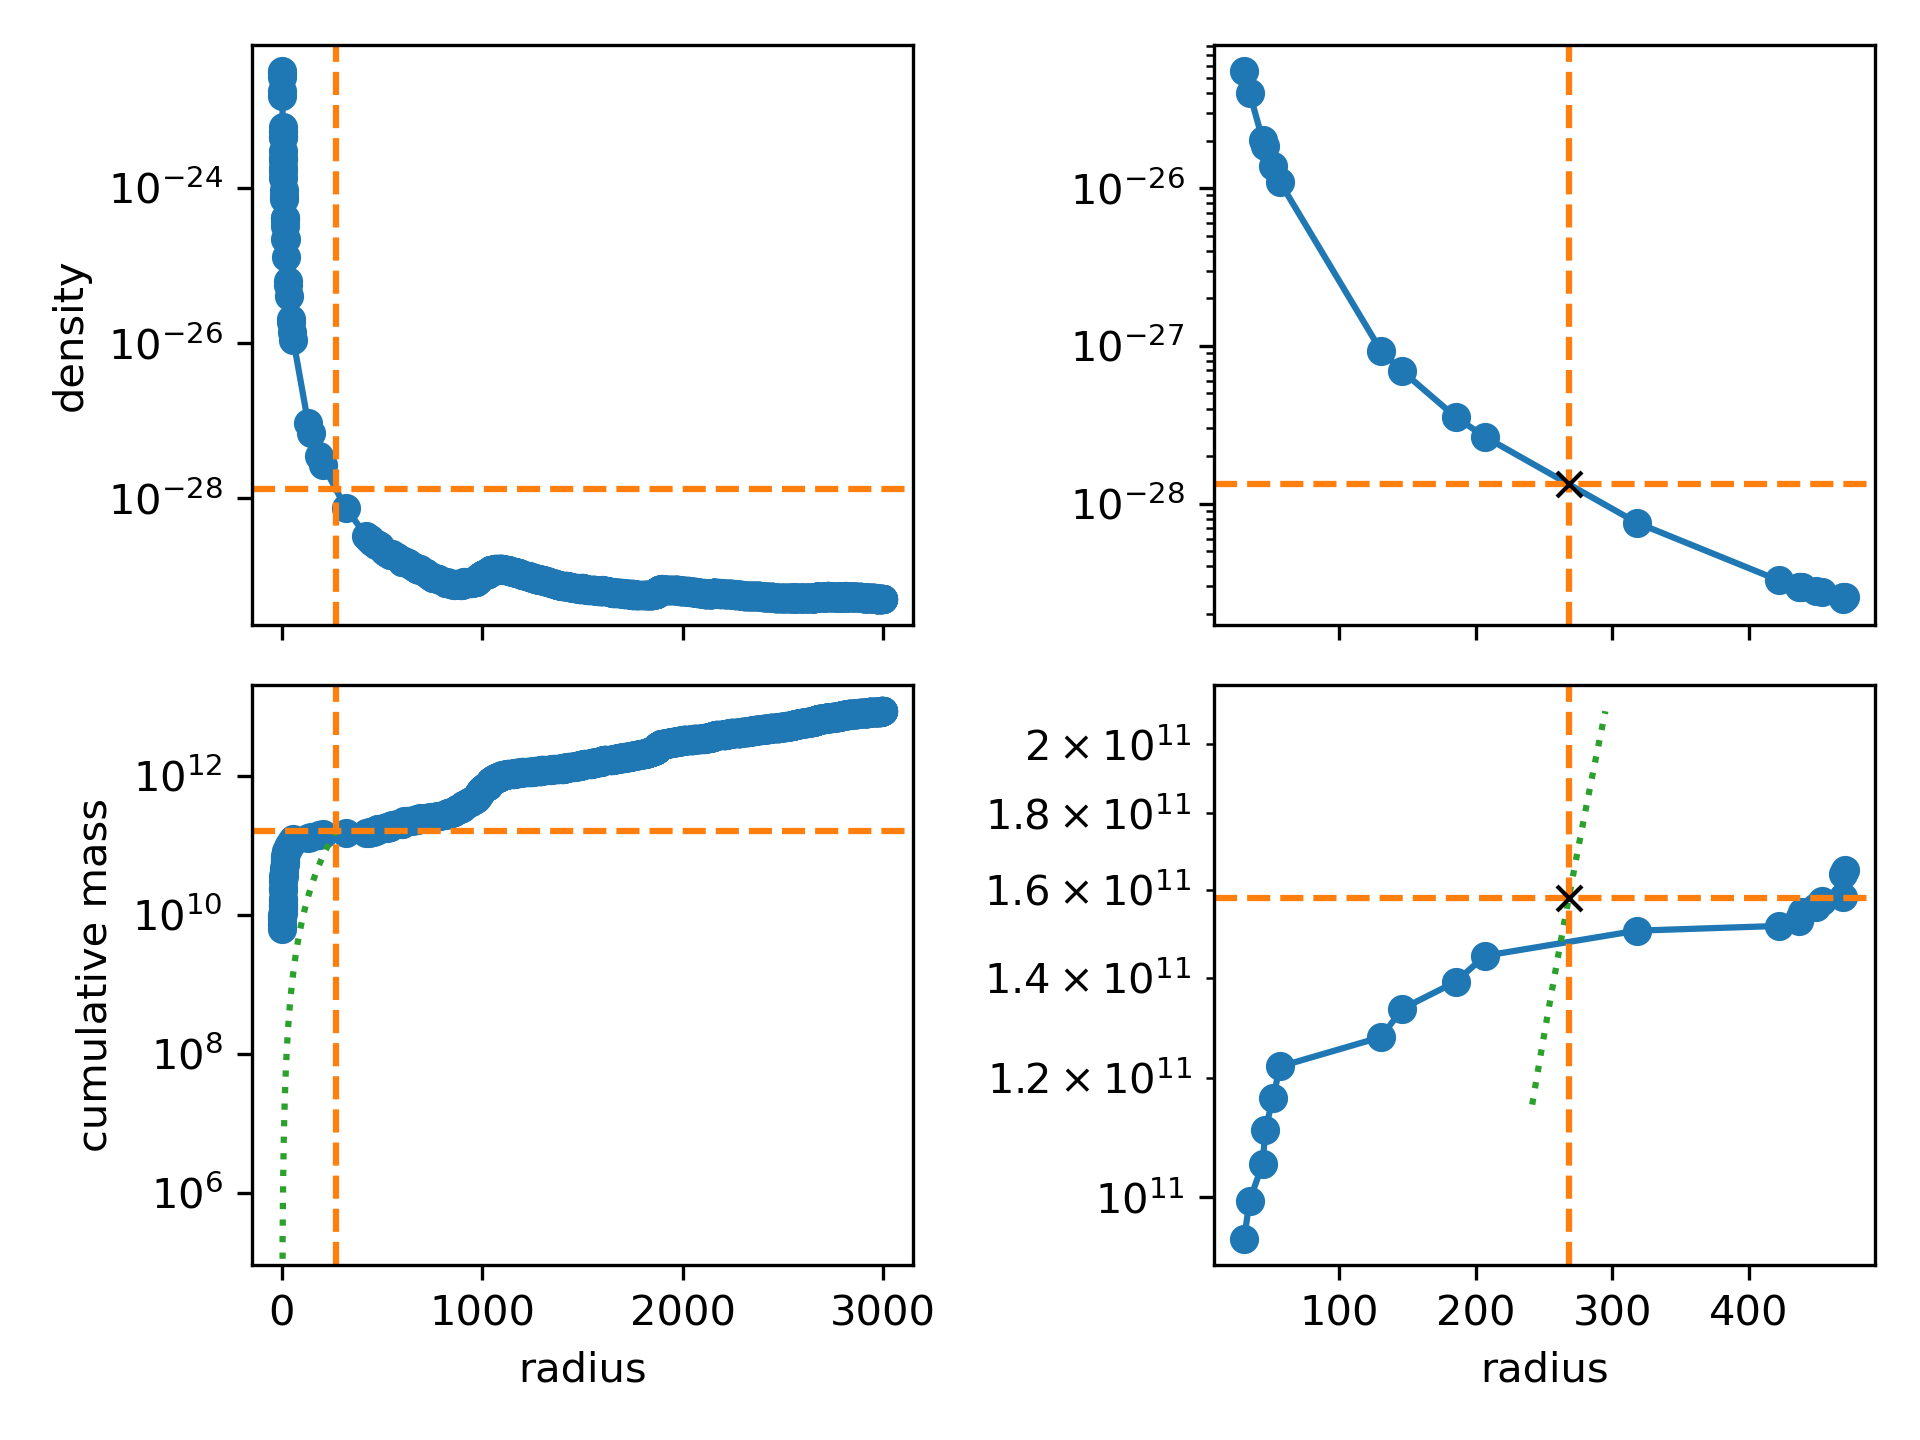
\includegraphics[width=0.48\textwidth{}]{image7.png}
    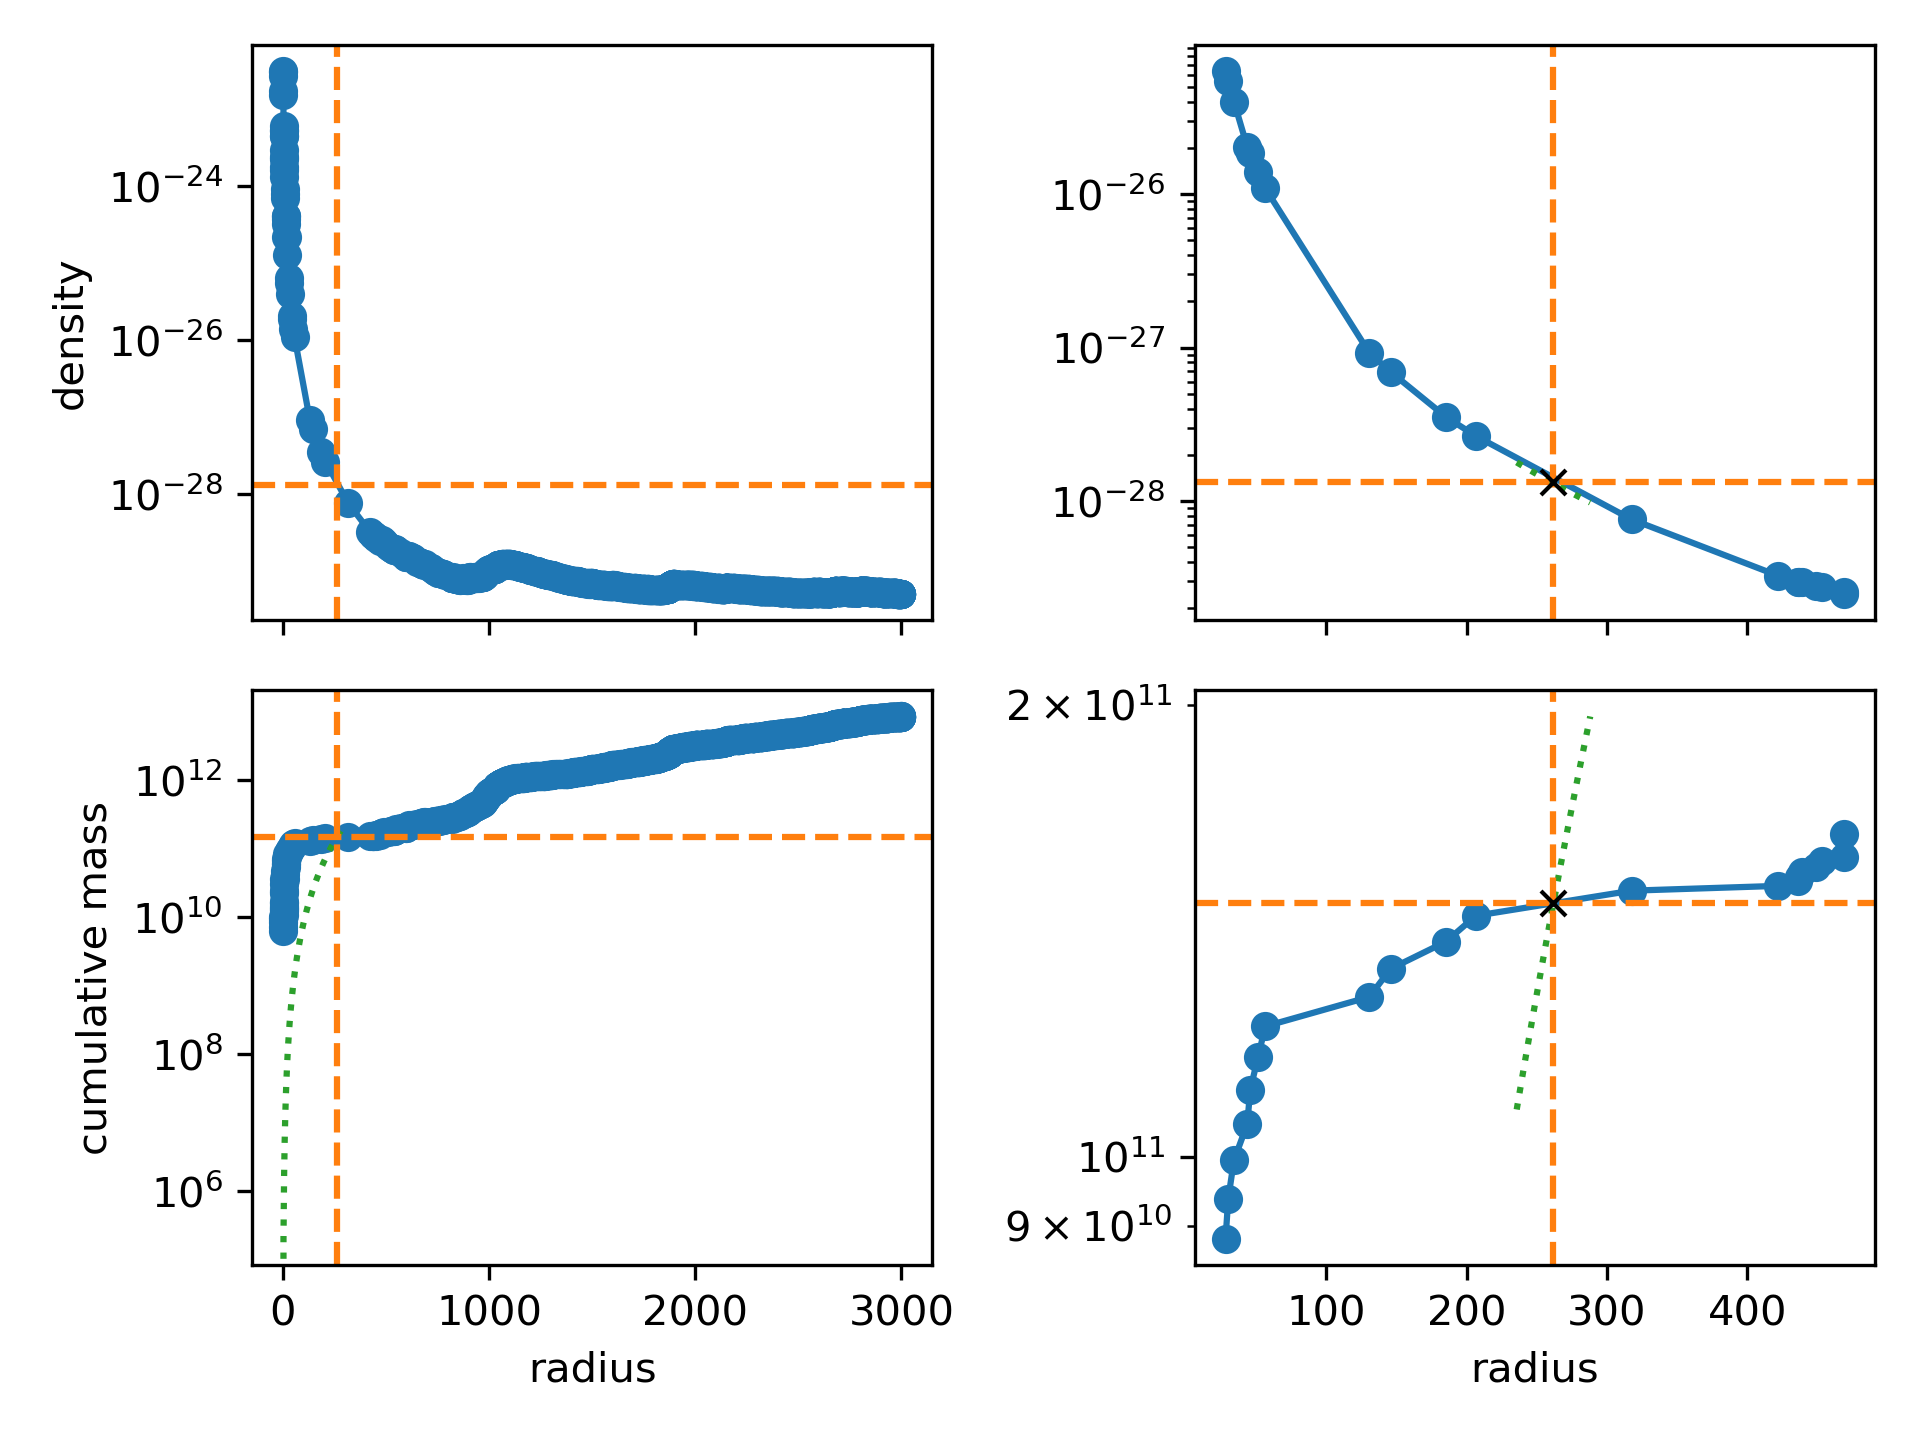
\includegraphics[width=0.48\textwidth{}]{image4.png}
    \caption{Density profile (\emph{top row}) and cumulative mass profile (\emph{bottom row}) for an example 
    halo in a 400 Mpc FLAMINGO box. The orange lines show $\rho{}_{\rm{}target}$ and $R_{\rm{}SO}$ and 
    $M_{\rm{}SO}$ as determined by SOAP, while the green line is the cumulative mass profile at fixed 
    $\rho{}_{\rm{}target}$. The two left columns correspond to a run where $R_{\rm{}SO}$ is fixed by 
    interpolating on the density profile (so in the top row plot), while the second two columns determine 
    $R_{\rm{}SO}$ by interpolating on the cumulative mass in the bottom row plots. The right column for each 
    pair of columns shows a zoom of the left column.}
    \label{fig:MSO_vs_RSO}
\end{figure}

While the interpolation of the logarithmic density profile to find $R_{\rm{}SO}$ is more straightforward, we 
found that it can lead to significant deviations between the value of $M_{\rm{}SO}$ and the cumulative mass in 
neighbouring bins that can be more than one particle mass, as illustrated in Fig. \ref{fig:MSO_vs_RSO}. The 
reason for this is that the cumulative mass profile at fixed density increases very steeply with radius, so 
that a small difference in $R_{\rm{}SO}$ leads to a relatively large difference in $M_{\rm{}SO}$. Conversely, 
fixing $M_{\rm{}SO}$ will lead to an $R_{\rm{}SO}$ that only deviates a little bit from the $R_{\rm{}SO}$ 
found by interpolating the density profile. However, doing so requires us to find the intersection of the 
cumulative mass profile at fixed density (green line in Fig. \ref{fig:MSO_vs_RSO}) with the actual cumulative 
mass profile, which means solving the following equation:

\begin{equation}
    \frac{4\pi{}}{3} \rho{}_{\rm{}target} R_{\rm{}SO}^3 = M_{\rm{}low} + \left( \frac{M_{\rm{}high}-M_{\rm{}low}}{R_{\rm{}high} - R_{\rm{}low}} \right) \left(R_{\rm{}SO} - R_{\rm{}low}\right),
    \label{eq:RSO}
\end{equation}

where $R/M_{\rm{}low/high}$ are the bounds of the intersecting bin (which we find in the density profile). 
This third degree polynomial equation has no unique solution, although in practice only one of the three 
possible complex solutions is real. We find this solution by using a root finding algorithm within the 
intersecting bin (we use Brent's method for this).

For clarity, this is the full set of rules for determining the SO radius in SOAP:
\begin{enumerate}
    \item Sort particles according to radius and construct the cumulative mass profile.
    \item Discard any particles at zero radius, since we cannot compute a density for those. The mass of these 
    particles is used as an $r=0$ offset for the cumulative mass profile. Since the halo's centre is the 
    position of the most bound particle, there should always be at least one such particle.
    \item Construct the density profile by dividing the cumulative mass at every radius by the volume of the 
    sphere with that radius.
    \item Find intersection points between the density profile and the target density, i.e. the radii 
    $R_{1,2}$ and masses $M_{1,2}$ where the density profile goes from above to below the threshold:
    \begin{enumerate}
        \item If there are none, analytically compute $R_{\rm{}SO}=\sqrt{3M_1/(4\pi{}R_1\rho_{\rm{}target})}$, 
        where $R_1$ and $M_1$ are the first non zero radius and the corresponding cumulative mass. This is a 
        special case of Eq. (\ref{eq:RSO}). Unless there are multiple particles at the exact halo centre 
        position, this radius estimate will then be based on just two particles.
        \item In all other cases, we use $R_{1,2}$ and $M_{1,2}$ as input for Eq. (\ref{eq:RSO}) and solve for 
        $R_{\rm{}SO}$. The only exception is the special case where $R_1 = R_2$. If that happens, we simply 
        move further down the line until we find a suitable interval.

    \end{enumerate}
    \item From $R_{\rm{}SO}$, we determine $M_{\rm{}SO}$ using Eq. (\ref{eq:MSO_condition}).
\end{enumerate}

\paragraph{Neutrinos -- if present in the model -- are included} in the inclusive sphere calculation (and only 
here, since neutrino particles cannot be bound to a halo) by adding both their weighted masses (which can be 
negative), as well as the contribution from the background neutrino density. The latter is achieved by 
explicitly adding the cumulative mass profile at constant neutrino density to the total cumulative mass 
profile before computing the density profile. This is the only place where neutrinos explicitly enter the 
algorithm, except for the neutrino masses computed for the SOs. Neutrinos are not included in the calculation 
of the centre of mass and centre of mass velocity.

\section{Group membership files}

Before SOAP can be run we generate a set of files which contain halo
membership information for each particle in the SWIFT snapshot. The
datasets in these files are stored in the same order and with the same
partitioning between files as the datasets in the snapshots. This
allows SOAP to read halo membership information for sub-regions of the
simulation volume without reading the full halo-finder output. These files may
also be useful for visualising the input halo catalogue.

The group membership files are HDF5 files with one group for each
particle type, named PartType0, PartType1, ... as in the
snapshots. Each group contains the following datasets:

\begin{enumerate}
\item \verb|GroupNr_bound|: for each particle in the corresponding snapshot
  file this contains the index in the original halo finder catalogue of the object 
  which the particle is bound to. Note this is not the same as the index of the object
  in the SOAP catalogue, it instead corresponds to the value of \verb|HaloCatalogueIndex|
  stored in the SOAP catalogues. If a particle is not bound to any subhalo it
  will have \verb|GroupNr_bound|=-1.
\item \verb|Rank_bound|: the ranking by total energy of this particle within
  the subhalo it belongs to, or -1 if the particle is not bound to
  any subhalo. The particle with the most negative total energy has
  \verb|Rank_bound|=0.
\item \verb|FOFGroupIDs|: the 3D FOF group the particle is part of.
  This field is only present if a FOF snapshot is listed in the
  parameter file. This field is present in the snapshots themselves,
  but for FLAMINGO hydro simulations the FOF was regenerated. If this
  field is present it will overwrite the value from the snapshots when
  SOAP is run.
\end{enumerate}

The script \verb|make_virtual_snapshot.py| will combine snapshot and group membership files
into a single virtual snapshot file. This virtual file can be read by swiftsimio and 
gadgetviewer to provide halo membership information alongside other particle properties.
Using the virtual file along with the spatial masking functionality within swiftsimio
means it is possible to quickly load all the particles bound to a given subhalo.
The \href{https://swiftgalaxy.readthedocs.io/en/latest/index.html}{SWIFTGalaxy package}
makes use of the membership files, and is helpful for analysing individual galaxies when 
manipulating their particles (recentering, rotations, cylindrical coordinates, etc.).

\end{document}
